%! TEX root = main.tex

\graphicspath{{00_Images/04_chapter/}}

\chapter{Active Balanced Inputs - CMRR Improvement}
\label{ch:cmrr}

\section{Source Impedance Problem and Differential Amplifier}
\label{sc:41}

The standard single-Op-Amp differential amplifier with four matched resistors achieves its ideal Common-Mode Rejection Ratio (CMRR) only when the gain seen by the non-inverting path equals the gain seen by the inverting path.
To make this condition explicit, consider the individual gains:
\[
    |G^+| = \left|\frac{v_{out}}{v_1}\right|_{v_2=0} = \left|1 + \frac{R_2}{R_1}\right|,
    \qquad
    |G^-| = \left|\frac{v_{out}}{v_2}\right|_{v_1=0} = \left|\frac{R_2}{R_1}\right|
\]
The differential and common-mode gains are:
\[
    G_{DIFF} = \frac{G^+ + G^-}{2}, \qquad G_{CM} = G^+ - G^-
\]
and perfect rejection requires \(G^+ = G^-\), which drives \(G_{CM} = 0\) and \(\mathrm{CMRR} \to \infty\).

\begin{figure}[!htb]
    \centering
    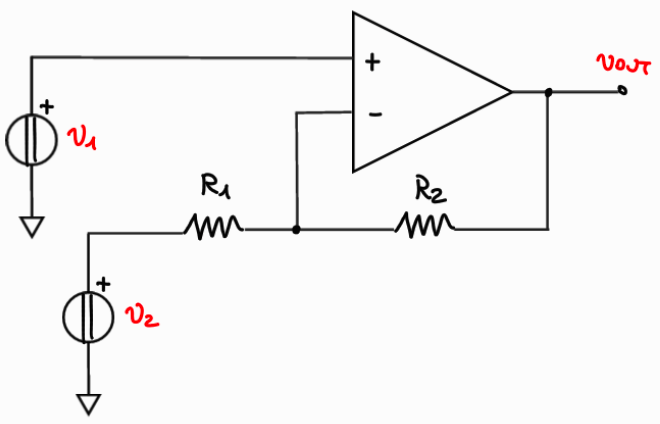
\includegraphics[width=0.90\textwidth]{OPAMP_FB_Config.png}
    \caption{Standard single-Op-Amp differential amplifier. With perfectly matched resistors \(R_1\) and \(R_2\) the common-mode gain \(G_{CM}\) is zero and the CMRR is theoretically infinite; any mismatch or unequal source impedances immediately degrades the rejection}
    \label{fig:diffAmp}
\end{figure}

In practice the condition \(G^+ = G^-\) can be violated for two independent reasons: resistor mismatch within the feedback network, and unequal source impedances \(R_{S1} \neq R_{S2}\) at the two inputs.
The second cause is examined here because it is inherent to the physical world and cannot be eliminated by better component matching alone.

\subsection{Effect of Unequal Source Impedances}

Real signal sources are not ideal voltage generators: they present finite output (source) impedances \(R_{S1}\) and \(R_{S2}\) in series with the two input lines.
These impedances become part of the voltage dividers that determine the effective gains, as shown in figure \ref{fig:sourceImp}.

\begin{figure}[!htb]
    \centering
    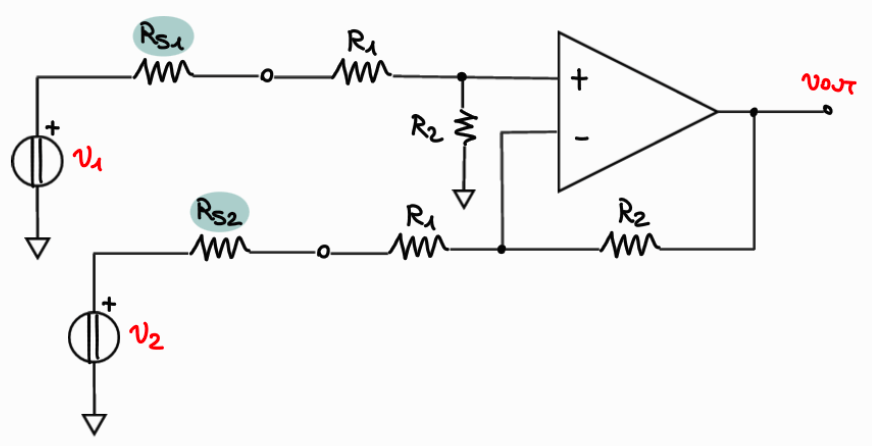
\includegraphics[width=0.90\textwidth]{OPAMP_FB_Correct_Source_Imp.png}
    \caption{Differential amplifier driven by sources with finite impedances \(R_{S1}\) and \(R_{S2}\). The asymmetry \(R_{S1} \neq R_{S2}\) unbalances the two signal paths, introducing a non-zero common-mode gain even when the four amplifier resistors are perfectly matched}
    \label{fig:sourceImp}
\end{figure}

\paragraph{Computing \(G^-\)} With \(v_1 = 0\), the inverting node carries the current from \(v_2\) through the series combination of \(R_{S2}\) and \(R_1\).
Applying the virtual short circuit (\(i^- = 0\)):
\[
    \frac{v_2}{R_1 + R_{S2}} + \frac{v_{out}}{R_2} = 0
    \quad\Longrightarrow\quad
    G^- = -\frac{R_2}{R_1 + R_{S2}}
\]

\paragraph{Computing \(G^+\)} With \(v_2 = 0\), the non-inverting input voltage is set by the voltage divider formed by \(R_{S1}\) and the parallel combination of \(R_2\) with the series \((R_1 + R_{S2})\):
\[
    v^+ = v_1 \cdot \frac{R_2}{R_1 + R_{S1} + R_2}
\]
The virtual short circuit gives \(v^- = v^+\), and writing the inverting node equation yields:
\[
    G^+ = \frac{R_2}{R_1 + R_{S2}} \cdot \frac{R_1 + R_2 + R_{S2}}{R_1 + R_2 + R_{S1}}
\]

\paragraph{Condition for \(|G^+| = |G^-|\)} Setting \(|G^+| = |G^-|\) requires:
\[
    \frac{R_1 + R_2 + R_{S2}}{R_1 + R_2 + R_{S1}} = 1
    \quad\Longrightarrow\quad
    R_{S1} = R_{S2}
\]
The CMRR is therefore preserved only when the two source impedances are identical.
This is a condition that cannot be guaranteed in practice: microphone output impedances vary with frequency and between units, cable resistance is asymmetric in unbalanced connections, and any real balanced source exhibits a finite impedance mismatch between its two output terminals.
Even a \SI{10}{\ohm} difference between \(R_{S1}\) and \(R_{S2}\) is sufficient to reduce the CMRR of a nominally high-performance stage from the ideal infinite value to a finite and potentially audible level.

\section{Buffer-Based Improvement}
\label{sc:42}

The simplest way to remove the source impedances from the gain equations is to insert a unity-gain voltage buffer at each input before the differential amplifier, as shown in figure \ref{fig:bufferCMRR}.
Because ideal buffers have infinite input impedance and zero output impedance, the voltages at the differential amplifier inputs are exact copies of the source voltages, independent of \(R_{S1}\) and \(R_{S2}\).
The sensitivity of \(G^+\) and \(G^-\) to source impedance mismatch is therefore eliminated.

\begin{figure}[!htb]
    \centering
    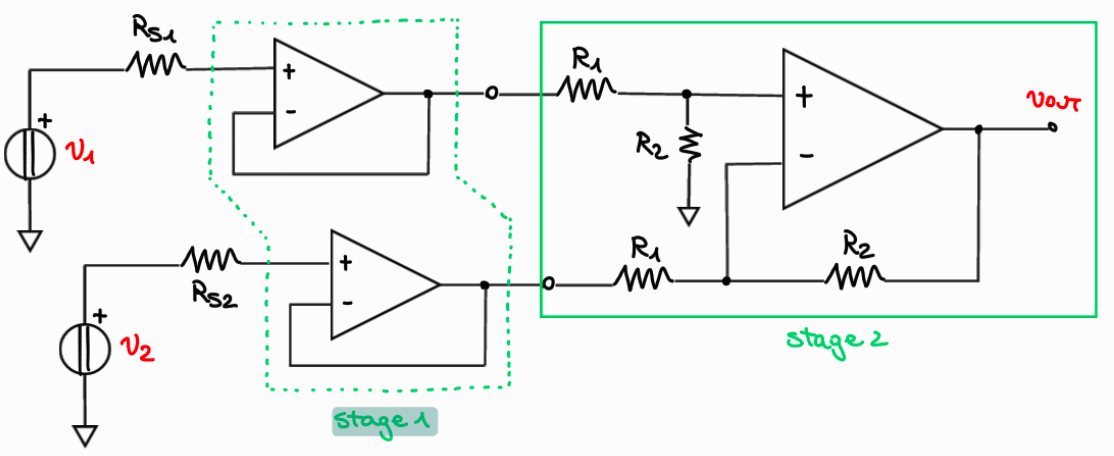
\includegraphics[width=0.90\textwidth]{CMRR_Improvement_Buffers.png}
    \caption{Two-stage architecture with input voltage buffers followed by the differential amplifier. The buffers isolate the source impedances from the signal path, so the second-stage CMRR is determined solely by the resistor matching of the differential stage}
    \label{fig:bufferCMRR}
\end{figure}

The total CMRR of this two-stage architecture is:
\[
    \mathrm{CMRR}_{TOT} = \mathrm{CMRR}_{\text{stage 1}} \times \mathrm{CMRR}_{\text{stage 2}}
\]
The buffer stage contributes \(\mathrm{CMRR}_{\text{stage 1}} \approx 1\) (since unity-gain buffers have equal gains on both paths), so the overall rejection remains limited by the second stage.
The second stage still relies on the matching of its four resistors to achieve a high \(G_{DIFF}/G_{CM}\) ratio; in practice, component tolerances and the finite CMRR of the Op-Amp itself cap the achievable rejection.
The buffer solution therefore solves the source impedance problem but does not improve the inherent rejection capability of the differential amplifier itself.

\section{The Instrumentation Amplifier: Gain Stage Implementation}
\label{sc:43}

A more powerful solution replaces the input buffers with an actively cross-coupled gain stage that simultaneously amplifies the differential signal and maintains unity common-mode gain.
The resulting three-Op-Amp topology is the standard instrumentation amplifier (INA) used throughout professional audio and measurement equipment.

\subsection{First-Stage Analysis}

The first stage consists of two Op-Amps cross-coupled by three resistors \(R_3\), \(R_4\), and \(R_5\), as shown in figure \ref{fig:gainStage}.
Each Op-Amp drives one output (\(v_{o1}\) and \(v_{o2}\)), and the three resistors form a single current-carrying branch between the two Op-Amp outputs through the inverting inputs.

\begin{figure}[!htb]
    \centering
    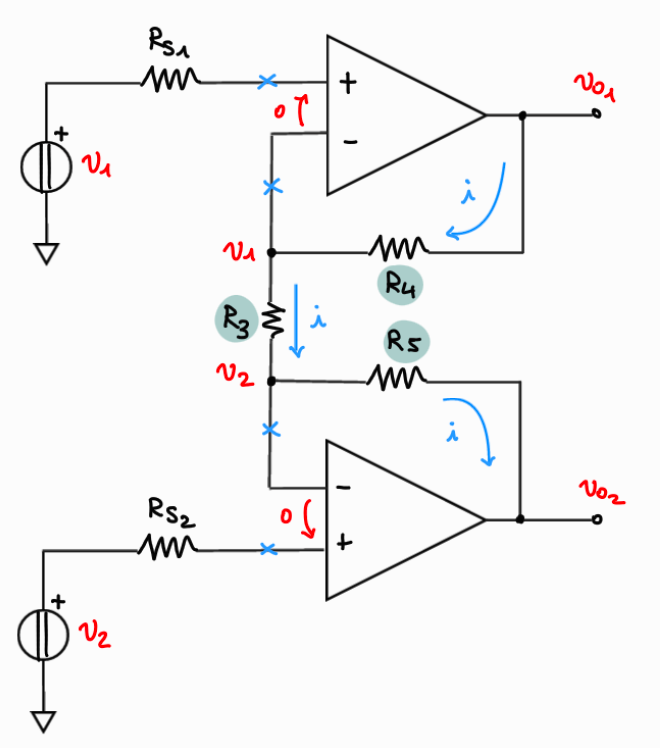
\includegraphics[width=0.90\textwidth]{CMRR_Improvement_Gain_Stage.png}
    \caption{Cross-coupled first stage of the instrumentation amplifier. The single current \(i\) flows through the branch \(R_4\text{--}R_3\text{--}R_5\); the virtual short circuit forces \(v^- = v^+ = v_{1,2}\) at each Op-Amp, so \(i\) is determined entirely by the differential voltage \(v_1 - v_2\)}
    \label{fig:gainStage}
\end{figure}

Because the virtual short circuit forces the inverting input of each Op-Amp to equal its non-inverting input, the voltages at the two ends of \(R_3\) are exactly \(v_1\) and \(v_2\).
A single common current \(i\) therefore flows through the entire branch:
\[
    v_{o1} - v_1 = R_4 i, \qquad v_1 - v_2 = R_3 i, \qquad v_2 - v_{o2} = R_5 i
\]
From the central equation:
\[
    i = \frac{v_1 - v_2}{R_3}
\]
Substituting back:
\[
    v_{o1} = v_1\left(1 + \frac{R_4}{R_3}\right) - \frac{R_4}{R_3} v_2,
    \qquad
    v_{o2} = v_2\left(1 + \frac{R_5}{R_3}\right) - \frac{R_5}{R_3} v_1
\]

\subsection{First-Stage Differential and Common-Mode Gains}

\paragraph{Differential gain} Subtracting the two output expressions:
\[
    v_{DIFF,out} = v_{o1} - v_{o2}
    = v_1\left(1 + \frac{R_4+R_5}{R_3}\right) - v_2\left(1 + \frac{R_4+R_5}{R_3}\right)
\]
\[
    v_{DIFF,out} = G_{DIFF,1}\cdot(v_1 - v_2), \qquad G_{DIFF,1} = 1 + \frac{R_4 + R_5}{R_3}
\]

\paragraph{Common-mode gain} Starting from the individual output expressions and taking the average:
\[
    v_{CM,out} = \frac{v_{o1} + v_{o2}}{2}
    = \frac{1}{2}\left[v_1\left(1 + \frac{R_4 - R_5}{R_3}\right) + v_2\left(1 + \frac{R_5 - R_4}{R_3}\right)\right]
\]
Setting \(R_4 = R_5\) makes every term containing \((R_4 - R_5)/R_3\) vanish, giving:
\[
    v_{CM,out} = \frac{v_1 + v_2}{2} \quad\Longrightarrow\quad G_{CM,1} = 1
\]
The first stage therefore amplifies the differential component by \(G_{DIFF,1} > 1\) while passing the common-mode component at unity gain.

\subsection{Overall CMRR}

The total CMRR of the complete instrumentation amplifier is:
\[
    \mathrm{CMRR}_{TOT} = \mathrm{CMRR}_{\text{stage 1}} \times \mathrm{CMRR}_{\text{stage 2}}
\]
where:
\[
    \mathrm{CMRR}_{\text{stage 1}} = \frac{G_{DIFF,1}}{G_{CM,1}} = G_{DIFF,1} = 1 + \frac{R_4 + R_5}{R_3}
\]
Since \(\mathrm{CMRR}_{\text{stage 1}} > 1\), the overall rejection always exceeds that of the differential stage alone:
\[
    \mathrm{CMRR}_{TOT} = G_{DIFF,1} \cdot \mathrm{CMRR}_{\text{stage 2}} > \mathrm{CMRR}_{\text{stage 2}}
\]

\begin{figure}[!htb]
    \centering
    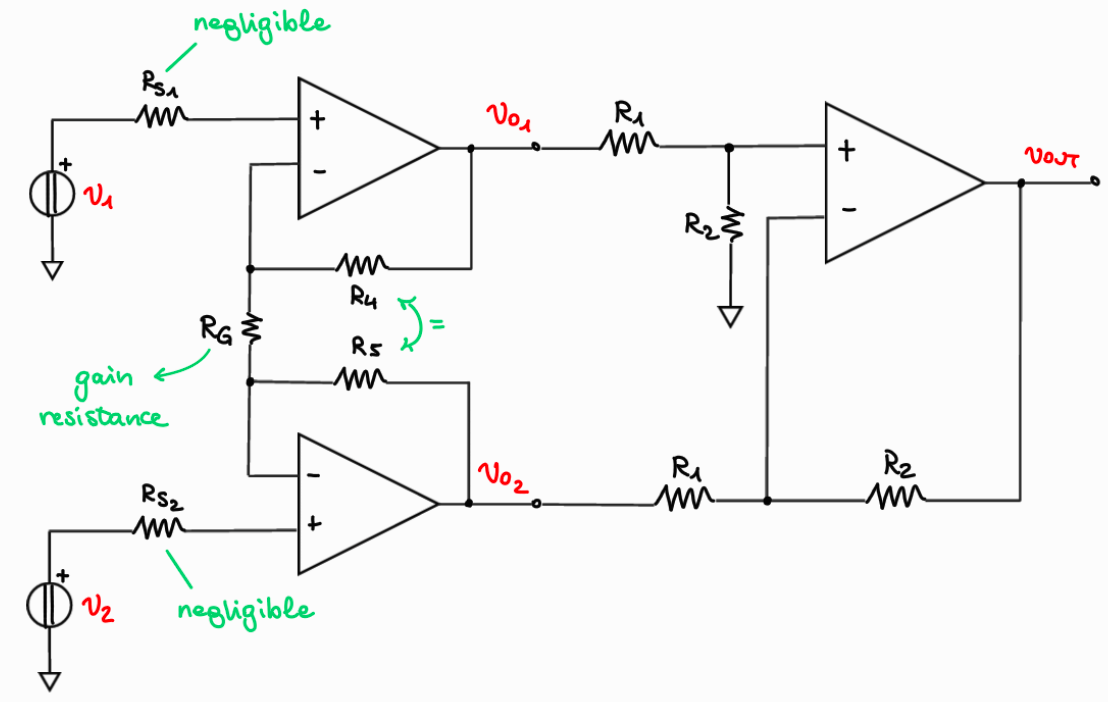
\includegraphics[width=0.90\textwidth]{CMRR_Improvement_Final_Scheme.png}
    \caption{Complete three-Op-Amp instrumentation amplifier. The cross-coupled first stage boosts the differential gain while maintaining unity common-mode gain; the standard differential second stage provides additional common-mode rejection. The overall CMRR is the product of the two stage CMRRs}
    \label{fig:finalINA}
\end{figure}

A crucial practical feature of this architecture is that the differential gain \(G_{DIFF,1}\), and therefore the overall amplifier gain, depends only on the single resistor \(R_3\) (often labeled \(R_G\) in commercial devices).
Changing \(R_3\) scales \(G_{DIFF,1}\) without disturbing the balance between \(R_4\) and \(R_5\), which means the common-mode gain \(G_{CM,1} = 1\) is maintained regardless of the chosen gain setting.
In a standard differential amplifier, adjusting the gain requires changing the ratio of matched resistor pairs simultaneously, inevitably introducing mismatch and degrading the CMRR.
In the instrumentation amplifier topology, the gain and the balance are decoupled: a single resistor controls the gain while the CMRR is protected by the fixed symmetry \(R_4 = R_5\).
This is the fundamental reason why the three-Op-Amp instrumentation amplifier is the standard architecture for high-performance balanced audio inputs, measurement front-ends, and any application where both high gain and high common-mode rejection are simultaneously required.
